\documentclass[12pt]{article}
\usepackage{geometry}
\usepackage{graphicx}
\usepackage{xcolor}
\renewcommand{\familydefault}{\sfdefault}
\usepackage{helvet}
\title{PHC 6000: Homework 2}
\author{Joe Brew}
\usepackage{Sweave}
\begin{document}
\newgeometry{margin=1.5cm}
\Sconcordance{concordance:homework2.tex:homework2.Rnw:%
1 8 1 1 0 20 1 1 2 1 0 1 1 3 0 1 2 31 1 1 2 1 0 3 1 1 2 1 1 1 2 1 3 1 0 %
1 2 1 1 4 0 1 3 8 1 1 2 1 0 3 1 1 2 1 1 2 2 2 1 3 0 1 2 10 1 1 2 1 0 3 %
1 1 2 2 1 1 2 1 1 1 2 2 1 1 2 2 1 3 0 1 2 7 1 1 12 1 2 26 1}

\maketitle
\begin{center}
UF-ID: 0402-8902\\
\noindent Joseph.Brew@FLHealth.gov
\end{center}

\vspace{30mm}
\tableofcontents

\newpage
\section*{Problem 1: Disability and Rurality}
\addcontentsline{toc}{section}{Problem 1: Disability and Rurality}
\textcolor{black!50}{As working in a project for a disability epidemiology course, MPH students A and B analyzed data from special survey sin Missouri adapted from the Behaviorial Risk Factor Surveillance System (BRFSS).  These were random digit dialed telphone surveys conducted in six Missouri counties between 1995 and 1997.  The sample consisted of a total of 3,343 adults: 1,380 from rural and 1,963 from nonrural areas.  Disability was defined as "limited in any way in any activities because of any impairment or health problem."  They hypothesized that disability would be increased in rural areas.} 

\subsection*{A}

\textcolor{black!50}{The table below shows the crude results of the study.  What kind of study is this?  Is there an increased prevalence of disability in rural areas compared to ruban areas? \\}

\begin{Schunk}
\begin{Sinput}
> prevRural <- 344 / (1036+344)
> prevUrban <- 444/(1519+444)
\end{Sinput}
\end{Schunk}


\noindent This is an \textbf{ecological} study.\\
There is indeed an increased prevalence of disability in rural areas (24.93\%) compared to urban areas (22.62\%).



\subsection*{B}
\textcolor{black!50}{What kind of study design would make the causal inference stronger for this hypothesis?  Since we cannot assign people randomly to their geographic residence, this will have to be an observational design.} \\


\noindent To make the causal inference stronger for the hypothesis that rurality increases disability, the ideal study design would be a \textbf{prospective cohort study}.  Though time-consuming (and perhaps expensive), this would allow the researcher to best parse out the effect of rurality on the risk of disability.

\section*{Problem 2: Air pollution and lung cancer}
\addcontentsline{toc}{section}{Problem 2: Air pollution and lung cancer}

\textcolor{black!50}{At a recent general science meeting you attended, the topic of discussion was the methods of measuring particulate matter in air pollution.  The author underscores her presentation about the importance of air pollution by reporting that she has seen cancer maps where it is clear that lung cancer varies as a function of population density and air pollution.  She concludes that air pollution, which is largely due to vehicular emissions, is a strong predictor of lung cancer by the maps' analysis of geographic areas.}  \\

\noindent\textcolor{black!50}{What concerns do you have about the type of study and the strengths of the evidence she cites?}\\



\noindent This is a textbook case of "ecological fallacy", in which the author infers that an individual's risk of an outcome (in this case, lung cancer) is high due to specific causes (population density, air pollution) which were gathered at the \textbf{population} level.  \\

\noindent A second problem with this evidence is that it does not account for the potential for \textbf{confounding}.  Though it may be true that urban-dwellers are at a higher risk for lung cancer, this may be due to a variety of other factors (age, smoking, occupation  etc.) which are not addressed in the author's evidence. 

\newpage
\section*{Problem 3: Aspirin and MI}
\addcontentsline{toc}{section}{Problem 3: Aspirin and MI}

\textcolor{black!50}{Physicians enrolled in they Physician's Health Study were randomly assigned to take a daily aspirin or placebo.  The table provides the number with MI in each group.  Calculate the RR and 95\% CI for the RR for MI (aspiring group compared to placebo group) and interpret the results.  \\}

\begin{Schunk}
\begin{Sinput}
> prob3 <- as.data.frame(c("aspirin", "placebo"))
> colnames(prob3) <- "group"
> prob3$yes <- c(139, 239)
> prob3$no <- c(10898, 10795)
> aspirinRisk <- prob3$yes[which(prob3$group == "aspirin")] / 11037
> placeboRisk <- prob3$yes[which(prob3$group == "placebo")] / 11034
> relativeRisk <- aspirinRisk/placeboRisk
> #SE(ln(RR))=sqrt (1/O0+1/O1)
> selnrr <- sqrt((1/139) - (1/11037) + (1/239) - (1/11034))
> ciHigh <- exp(log(relativeRisk) + 1.96*selnrr)
> ciLow <- exp(log(relativeRisk) - 1.96*selnrr)
> 
\end{Sinput}
\end{Schunk}

\noindent Compared to those on a placebo, study participants taking aspirin had a relative risk (RR) of 0.5814 for Myocardial Infarction (MI).  This means that, at a 95\% confidence level, those taking aspirin had a 41.86\% lower risk of MI compared to those on a placebo (95\% confidence interval of 0.47, 0.72).  \\

\noindent In laymen's terms, we are 95\% confident that the true reduction in risk is between 0.47\% and 0.72\%. 

\section*{Problem 4: Preterm delivery and SES}
\addcontentsline{toc}{section}{Problem 4: Preterm delivery and SES}

\textcolor{black!50}{A case-control study of the epidemiology of preterm delivery was undertaken at Yale-New Haven Hospital in Connecticut during 1977.  The table on the following slide contains data for the Mother's socioeconomic status (SES) for those with (cases) and without (controls) preterm delivery.  Calculate OR and corresponding 95\% Confidence Interval for preterm delivery comparing Lower to Upper SES and interpret your findings.  \\}
\begin{Schunk}
\begin{Sinput}
> prob4 <- as.data.frame(c("lower", "upper"))
> colnames(prob4) <- "ses"
> prob4$yes <- c(53,11)
> prob4$no <- c(58,40)
> oddsCases <- 53/11
> oddsControls <- 58/40
> oddsRatio <- oddsCases/oddsControls
> selnor <- sqrt((1/53) + (1/58) + (1/11) + (1/40))
> ciHigh <- exp(log(oddsRatio)) + 1.96*selnor
> ciLow <- exp(log(oddsRatio)) - 1.96*selnor
\end{Sinput}
\end{Schunk}

\noindent Among those with pre-term birth (cases), the odds of being of lower socioeconomic status (relative to controls, those of upper SES) is 3.32.  The 95\% confidence interval is 2.56, 4.09.  In other words, the risk of pre-term birth is 2.5 to 4 times higher for mothers of low SES.  

\newpage


\section*{Problem 5: Alcohol consumption and esophageal cancer}
\addcontentsline{toc}{section}{Problem 5: Alcohol consumption and esophageal cancer}

\textcolor{black!50}{Data from a case-control study of 200 esophageal cancer cases and 775 community-based controls are shown below.  Detailed dietary data were obtained by interview.  This example addresses the relation between alcohol consumption (categorized as none, 1-50 g per day, and 50-80 grams per day) and esophageal cancer (Table below).  Using no alcohol consumption as a reference group, calculate ORs for each of teh alcohol consumption levels and interpret your findings.  \\}

\begin{Schunk}
\begin{Sinput}
> prob5 <- as.data.frame(c("high", "low", "none"))
> colnames(prob5) <- "alcohol"
> prob5$yes <- c(96, 85, 104)
> prob5$no <- c(109, 200, 666)
> oddsYesNone <- 104/666
> oddsYesLow <- 85/200
> oddsYesHigh <- 96/109
> oddsRatioLow <- oddsYesLow / oddsYesNone
> oddsRatioHigh <- oddsYesHigh / oddsYesNone
> selnorLow <- sqrt((1/85) + (1/200) + (1/104) + (1/666))
> ciLowLow <- exp(log(oddsRatioLow) - 1.96*selnorLow)
> ciLowHigh <- exp(log(oddsRatioLow) + 1.96*selnorLow)
> selnorHigh <- sqrt((1/96) + (1/109) + (1/104) + (1/666))
> ciHighLow <- exp(log(oddsRatioHigh) - 1.96*selnorHigh)
> ciHighHigh <- exp(log(oddsRatioHigh) + 1.96*selnorHigh)
\end{Sinput}
\end{Schunk}

\noindent This study suggests increased risk of esophageal cancer with increased alcohol consumption.  Study participants with esophageal cancer were 2.72 times more likely to consume 1-50 grams of alcohol per day (95\% confidence interval of 1.96, 3.78) than those without cancer.  \\

\noindent At greater levels of consumption, the risk increases.  Those with esophageal cancer were 5.64 time more likely to consume 50-80 grams of alcohol per day (95\% confidence interval of of 4, 7.95) than those without cancer. \\

\noindent A graphical display of this information is below:

\begin{center}
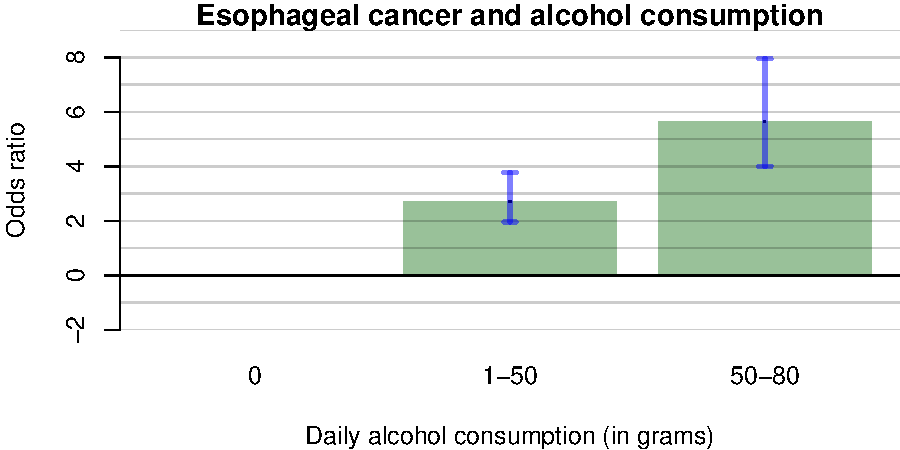
\includegraphics{homework2-005}
\end{center}
\newpage
\section*{Problem 6: Study designs}
\addcontentsline{toc}{section}{Problem 6: Study designs}

\textcolor{black!50}{For each of the following research questions, consider the issues of: \begin{enumerate}
\item frequency of the outcomes and exposures
\item the stage at which the question is directed (descriptive, hypothesis generating, hypothesis testing), and \\
\end{enumerate}
\noindent Suggest the \textbf{one "best" study design} and explain the reasons for your choice.  (Stick to cross-sectional, case-control, cohort, and experiments for these examples, unless you have a really compelling reason to select something else).} \\

\subsection*{A}
\textcolor{black!50}{The quality of life of persons with mental disorders, such as bipolar disorder, is unknown.  We are interested in describing the quality of life of persons with bipolar disorder and identify potential factors associated with an increase in perceived quality of life for a further study.}\\

\noindent A \textbf{cross-sectional} study would be the best design for this study.  Given that this is a somewhat "exploratory" study in the first place (it is not attempting to give evidence for causation or to link a certain exposure to a certain outcome), a cross-sectional design would help establish which exposures should be studied further.  

\subsection*{B}
\textcolor{black!50}{Cleft lip (with or without cleft palate) occurs in about 1 to 2 births per 1,000 in Northern European countries and in people of these backgrounds in the United States.  How would you investigate the hypothesis that a woman's exposure to certain medications during early pregnancy may increase the risk of these birth outcomes.}\\

\noindent A \textbf{case-control} design would be ideal for this study, given that the event (cleft lip) is rare.  A case-control would allow for the direct comparison of the odds of taking certain medications among those with the event and those without.  A prospective cohort study, although advantageous any many ways, would have to be enormous in order to get a meaningful number of cases.

\subsection*{C}
\textcolor{black!50}{A large number of people have been prescribed a medication for the treatment of depression.  One of the medications that has been prescribed the most is Prozac.  In standard clinical care, Prozac may be prescribed for long-term use.  However, very little is known of the long-term effects of taking Prozac.  We are interested in identifying what the effects of long-term Prozac use, such as the probability of relapse and the presence of side-effects, and what factors are associated with these events.}\\

\noindent A prospective \textbf{cohort} design is the ideal one for this study since we are interested in studying multiple outcomes (something which is not possible in a case-control).  

\end{document}
